\begin{figure}
	\hypertarget{fig:benchmarks}{%
	\centering
	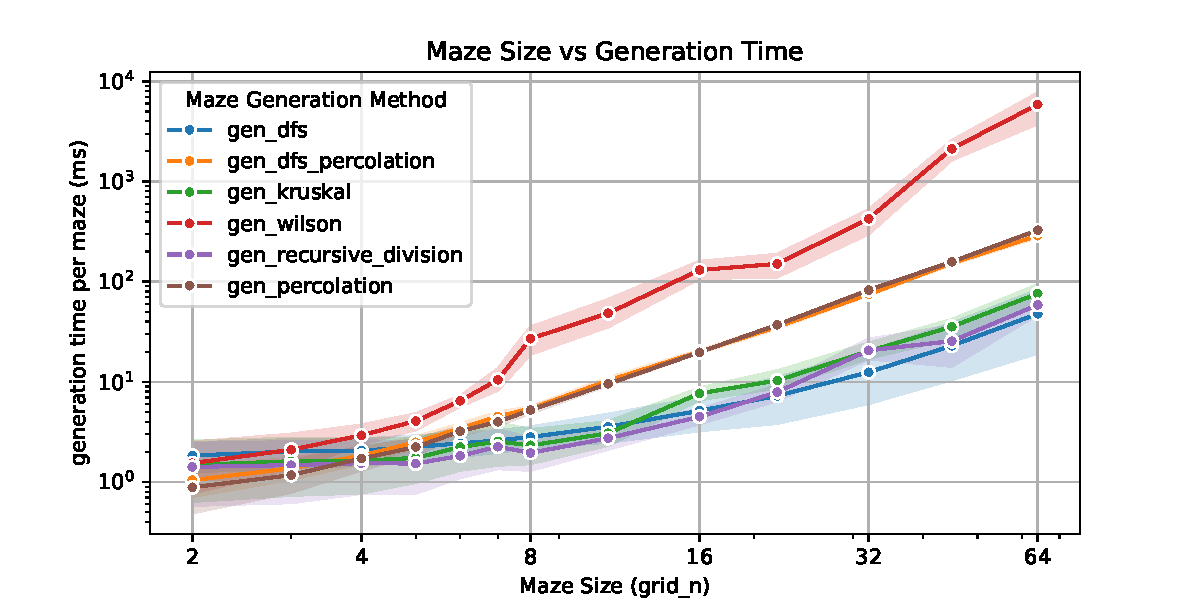
\includegraphics[width=0.9\textwidth,height=\textheight]{figures/benchmarks/gridsize-vs-gentime.pdf}
	\caption{Plot of maze generation time. Generation time scales
	exponentially with maze size for all algorithms. Generation time per
	maze does not depend on the number of mazes being generated, and there
	is minimal overhead to initializing the generation process for a small
	dataset. Wilson's algorithm is notably less efficient than others and
	has high variance. Note that values are averaged across all parameter
	sets for that algorithm. More information can be found on the
	\href{https://understanding-search.github.io/maze-dataset/benchmarks/}{benchmarks
	page}.}\label{fig:benchmarks}
	}
\end{figure}